\documentclass[a4paper,10pt]{article}
\usepackage[utf8x]{inputenc}
\usepackage{graphicx}

%opening
\title{}
\author{}

\begin{document}

\maketitle

\begin{abstract}
The Topic Browser is an open-source\footnote{Licensed under the terms of the Affero General Public License, version 3.}  web application for interactive exploration and visualization of topics and documents. Mallet LDA output is used as input. We explain why such a tool is warranted, what it is capable of, and how to use it to explore the corpus (or topic model) of your choice.
\end{abstract}

\section{Why?}
\subsection{Topic models are neat...}
Since their introduction in 2003, LDA-based topic models have been extended to account for time, authors, citations, multiple languages, etc. [][][][][] Baseline LDA generates a topic assignment per (non-stop) token -- a massive output in the gigaword era. Humans are incapable of fully assimilating the resulting models unaided, calling for more effective means of characterizing and visualizing the output. 

Previous visualization attempts....

Why they fail





\subsection{...but their output is hard for humans to digest}
\subsection{Topics aren't isolated entities, but form a network in combination with documents, words, authors, etc.}
\subsection{This network is implied by a topic model, but generally not made explicit (?)}
\subsection{More informative}
Experience suggests that an explicit representation of the relationships between all entities modeled and makes topic model output more informative and usable.
[We're in the process of formally validating this claim.]

\section{What?}
The Topic Browser is an open-source web application for interactive exploration and visualization of document collections. 

\subsection{Entities}
\begin{figure}[ht]
 \centering
 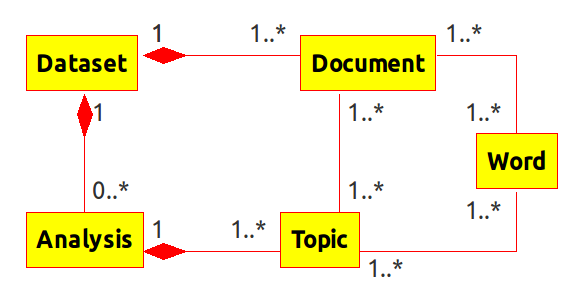
\includegraphics{topic_browser_object_model_transparent.png}
 % topic browser object model transparent.png: 582x293 pixel, 96dpi, 15.40x7.75 cm, bb=0 0 436 220
 \caption{The Topic Browser object model}
 \label{fig:object_model}
\end{figure}



All entities implied by topic model output are first-class citizens in the Topic Browser. 
Dataset->Document
Analysis->Topic
Word

\subsection{Topics}

\subsection{Documents}

\subsection{Words}

\subsection{Metrics}
topic, topic-topic, document, document-document

\subsection{Charts}

\subsection{Topic ``Maps"}
With topic-to-topic relationships described by means of pairwise topic metrics, graph-based visualization of the topic space becomes straightforward. In our current implementation, we construct a topic graph G = (N, E) as follows:
\begin{itemize}
\item $N$ is a set of $|T|$ nodes such that $\forall_{t\in T} weight(N_{t}) = \tau(t)$ where $\tau$ is a topic metric.
\item $E$ is a set of $|T|^2$ edges such that $\forall_{t\in T}\forall_{u\in T} weight(E_{t,u}) = \mu(t,u)$ where $\mu$ is a pairwise topic metric.
\end{itemize}

\subsection{Topic Name Schemes}


We use the Gephi Toolkit\footnote{http://www.gephi.org} to generate such graphs and render them as images. It 



\section{How?}
Describe how to import a document collection into TTB.


\end{document}
